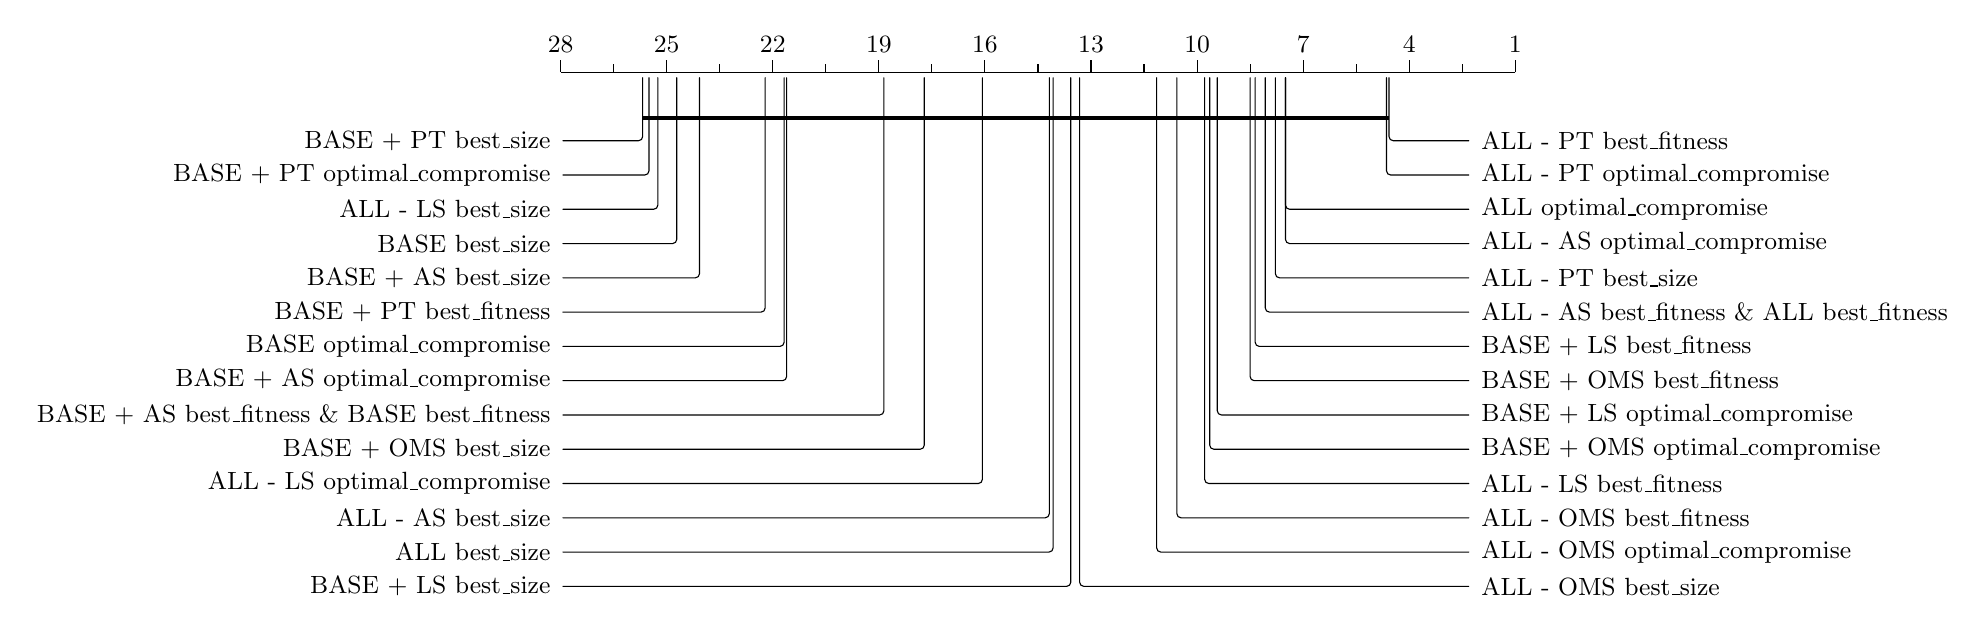
\begin{tikzpicture}[
  treatment line/.style={rounded corners=1.5pt, line cap=round, shorten >=1pt},
  treatment label/.style={font=\small},
  group line/.style={ultra thick},
]

\begin{axis}[
  clip={false},
  axis x line={center},
  axis y line={none},
  axis line style={-},
  xmin={1},
  ymax={0},
  scale only axis={true},
  width={\linewidth},
  ticklabel style={anchor=south, yshift=1.3*\pgfkeysvalueof{/pgfplots/major tick length}, font=\small},
  every tick/.style={draw=black},
  major tick style={yshift=.5*\pgfkeysvalueof{/pgfplots/major tick length}},
  minor tick style={yshift=.5*\pgfkeysvalueof{/pgfplots/minor tick length}},
  title style={yshift=\baselineskip},
  xmax={28},
  ymin={-15.5},
  height={16\baselineskip},
  xtick={1,4,7,10,13,16,19,22,25,28},
  minor x tick num={1},
  x dir={reverse},
]

\draw[treatment line] ([yshift=-2pt] axis cs:4.571428571428571, 0) |- (axis cs:2.2380952380952377, -2.0)
  node[treatment label, anchor=west] {ALL - PT best\_fitness};
\draw[treatment line] ([yshift=-2pt] axis cs:4.642857142857143, 0) |- (axis cs:2.2380952380952377, -3.0)
  node[treatment label, anchor=west] {ALL - PT optimal\_compromise};
\draw[treatment line] ([yshift=-2pt] axis cs:7.5, 0) |- (axis cs:2.2380952380952377, -4.0)
  node[treatment label, anchor=west] {ALL optimal\_compromise};
\draw[treatment line] ([yshift=-2pt] axis cs:7.5, 0) |- (axis cs:2.2380952380952377, -5.0)
  node[treatment label, anchor=west] {ALL - AS optimal\_compromise};
\draw[treatment line] ([yshift=-2pt] axis cs:7.785714285714286, 0) |- (axis cs:2.2380952380952377, -6.0)
  node[treatment label, anchor=west] {ALL - PT best\_size};
\draw[treatment line] ([yshift=-2pt] axis cs:8.071428571428571, 0) |- (axis cs:2.2380952380952377, -7.0)
  node[treatment label, anchor=west] {ALL - AS best\_fitness \& ALL best\_fitness};
\draw[treatment line] ([yshift=-2pt] axis cs:8.357142857142858, 0) |- (axis cs:2.2380952380952377, -8.0)
  node[treatment label, anchor=west] {BASE + LS best\_fitness};
\draw[treatment line] ([yshift=-2pt] axis cs:8.5, 0) |- (axis cs:2.2380952380952377, -9.0)
  node[treatment label, anchor=west] {BASE + OMS best\_fitness};
\draw[treatment line] ([yshift=-2pt] axis cs:9.428571428571429, 0) |- (axis cs:2.2380952380952377, -10.0)
  node[treatment label, anchor=west] {BASE + LS optimal\_compromise};
\draw[treatment line] ([yshift=-2pt] axis cs:9.642857142857142, 0) |- (axis cs:2.2380952380952377, -11.0)
  node[treatment label, anchor=west] {BASE + OMS optimal\_compromise};
\draw[treatment line] ([yshift=-2pt] axis cs:9.785714285714286, 0) |- (axis cs:2.2380952380952377, -12.0)
  node[treatment label, anchor=west] {ALL - LS best\_fitness};
\draw[treatment line] ([yshift=-2pt] axis cs:10.571428571428571, 0) |- (axis cs:2.2380952380952377, -13.0)
  node[treatment label, anchor=west] {ALL - OMS best\_fitness};
\draw[treatment line] ([yshift=-2pt] axis cs:11.142857142857142, 0) |- (axis cs:2.2380952380952377, -14.0)
  node[treatment label, anchor=west] {ALL - OMS optimal\_compromise};
\draw[treatment line] ([yshift=-2pt] axis cs:13.321428571428571, 0) |- (axis cs:2.2380952380952377, -15.0)
  node[treatment label, anchor=west] {ALL - OMS best\_size};
\draw[treatment line] ([yshift=-2pt] axis cs:13.571428571428571, 0) |- (axis cs:28.01190476190476, -15.0)
  node[treatment label, anchor=east] {BASE + LS best\_size};
\draw[treatment line] ([yshift=-2pt] axis cs:14.071428571428571, 0) |- (axis cs:28.01190476190476, -14.0)
  node[treatment label, anchor=east] {ALL best\_size};
\draw[treatment line] ([yshift=-2pt] axis cs:14.178571428571429, 0) |- (axis cs:28.01190476190476, -13.0)
  node[treatment label, anchor=east] {ALL - AS best\_size};
\draw[treatment line] ([yshift=-2pt] axis cs:16.071428571428573, 0) |- (axis cs:28.01190476190476, -12.0)
  node[treatment label, anchor=east] {ALL - LS optimal\_compromise};
\draw[treatment line] ([yshift=-2pt] axis cs:17.714285714285715, 0) |- (axis cs:28.01190476190476, -11.0)
  node[treatment label, anchor=east] {BASE + OMS best\_size};
\draw[treatment line] ([yshift=-2pt] axis cs:18.857142857142858, 0) |- (axis cs:28.01190476190476, -10.0)
  node[treatment label, anchor=east] {BASE + AS best\_fitness \& BASE best\_fitness};
\draw[treatment line] ([yshift=-2pt] axis cs:21.607142857142858, 0) |- (axis cs:28.01190476190476, -9.0)
  node[treatment label, anchor=east] {BASE + AS optimal\_compromise};
\draw[treatment line] ([yshift=-2pt] axis cs:21.678571428571427, 0) |- (axis cs:28.01190476190476, -8.0)
  node[treatment label, anchor=east] {BASE optimal\_compromise};
\draw[treatment line] ([yshift=-2pt] axis cs:22.214285714285715, 0) |- (axis cs:28.01190476190476, -7.0)
  node[treatment label, anchor=east] {BASE + PT best\_fitness};
\draw[treatment line] ([yshift=-2pt] axis cs:24.071428571428573, 0) |- (axis cs:28.01190476190476, -6.0)
  node[treatment label, anchor=east] {BASE + AS best\_size};
\draw[treatment line] ([yshift=-2pt] axis cs:24.714285714285715, 0) |- (axis cs:28.01190476190476, -5.0)
  node[treatment label, anchor=east] {BASE best\_size};
\draw[treatment line] ([yshift=-2pt] axis cs:25.25, 0) |- (axis cs:28.01190476190476, -4.0)
  node[treatment label, anchor=east] {ALL - LS best\_size};
\draw[treatment line] ([yshift=-2pt] axis cs:25.5, 0) |- (axis cs:28.01190476190476, -3.0)
  node[treatment label, anchor=east] {BASE + PT optimal\_compromise};
\draw[treatment line] ([yshift=-2pt] axis cs:25.678571428571427, 0) |- (axis cs:28.01190476190476, -2.0)
  node[treatment label, anchor=east] {BASE + PT best\_size};
\draw[group line] (axis cs:4.571428571428571, -1.3333333333333333) -- (axis cs:25.678571428571427, -1.3333333333333333);

\end{axis}
\end{tikzpicture}